\documentclass{beamer}
\usetheme{PaloAlto}
\usepackage{url}
\usepackage{latexsym}
\usepackage{graphicx}


% My Package Includes
\usepackage{upquote} % For real apostrophes (see http://tex.stackexchange.com/questions/63345/how-to-make-a-real-apostrophe-or-single-quote-in-latex#63348)
\usepackage{comment}
\usepackage{xcolor}
\definecolor{dark-blue}{rgb}{0.15,0.15,0.7}
\usepackage{hyperref}
%\hypersetup{colorlinks, linkcolor={dark-blue}, citecolor={dark-blue}, urlcolor={dark-blue}}
\hypersetup{colorlinks, linkcolor=black, citecolor=black, urlcolor=black}
\usepackage{booktabs}
\frenchspacing % Normal (single) spaces after periods.  Cf. http://www.read.seas.harvard.edu/~kohler/latex.html
%\usepackage{natbib}
\usepackage[shortcuts]{extdash} % use "\-/" to help LaTeX insert hyphen/pagebreaks
\usepackage[textwidth=0.9in]{todonotes}
\newcommand{\smalltodo}[2][]
    {\todo[caption={#2}, #1]
    {\tiny#2\normalsize}}


\newtheorem{requirement}{Requirement}



\begin{document}



\title[LingSync \& OLD] % (optional, use only with long paper titles)
{LingSync \& the Online Linguistic Database}



\author[~]{Joel Dunham \inst{1} \and Gina Cook \inst{2} \and Josh Horner \inst{3}}
\institute[UBC, LingSync.org]{\inst{1} University of British Columbia \and %
                      \inst{2} iLanguage Lab \and %
                      \inst{3} Amilia}


                      \subtitle
                      {New models for the collection and management of data for language communities, linguists and
                      language learners}

%\author[Author1,Author2] % (optional, use only with lots of authors)
%{Author One  \and Author Two }
% - Give the names in the same order as the appear in the paper.
% - Use the \inst{?} command only if the authors have different
%   affiliation.

% - Use the \inst command only if there are several affiliations.
% - Keep it simple, no one is interested in your street address.

\date[ComputEL 2014] % (optional, should be abbreviation of conference name)
{ComputEL Workshop, June 26 2014}



% \AtBeginSubsection[]
% {
% \setbeamertemplate{sidebar left}{}
%   \begin{frame}<beamer>
%     \frametitle{Outline}
%     \tableofcontents[currentsection,currentsubsection]
%   \end{frame}
%   \setbeamertemplate{sidebar left}[sidebar theme]
%
% }

\setbeamertemplate{sidebar left}{}
\begin{frame}
\titlepage
\end{frame}
\setbeamertemplate{sidebar left}[sidebar theme]

\section{Background}

\subsection[Fieldwork]{Endangered languages fieldwork}\label{sec:fieldwork}

\begin{frame}
Endangered languages fieldwork
\end{frame}

\subsection[Requirements]{Software requirements}

\begin{frame}


\begin{requirement}
\label{req:primary-data}
Integration of primary data
\end{requirement}


\begin{requirement}
\label{req:curation}
Curation of data
\end{requirement}


\begin{requirement}
\label{req:inclusive}
Inclusion of stakeholders
\end{requirement}

\begin{requirement}
\label{req:openable}
Openable data
\end{requirement}


\begin{requirement}
\label{req:productivity}
User productivity
\end{requirement}
\end{frame}


\subsection{Existing software}

\begin{frame}


%TODO will convert into latex diagrams once we are sure we want it.
\begin{figure}
\begin{center}
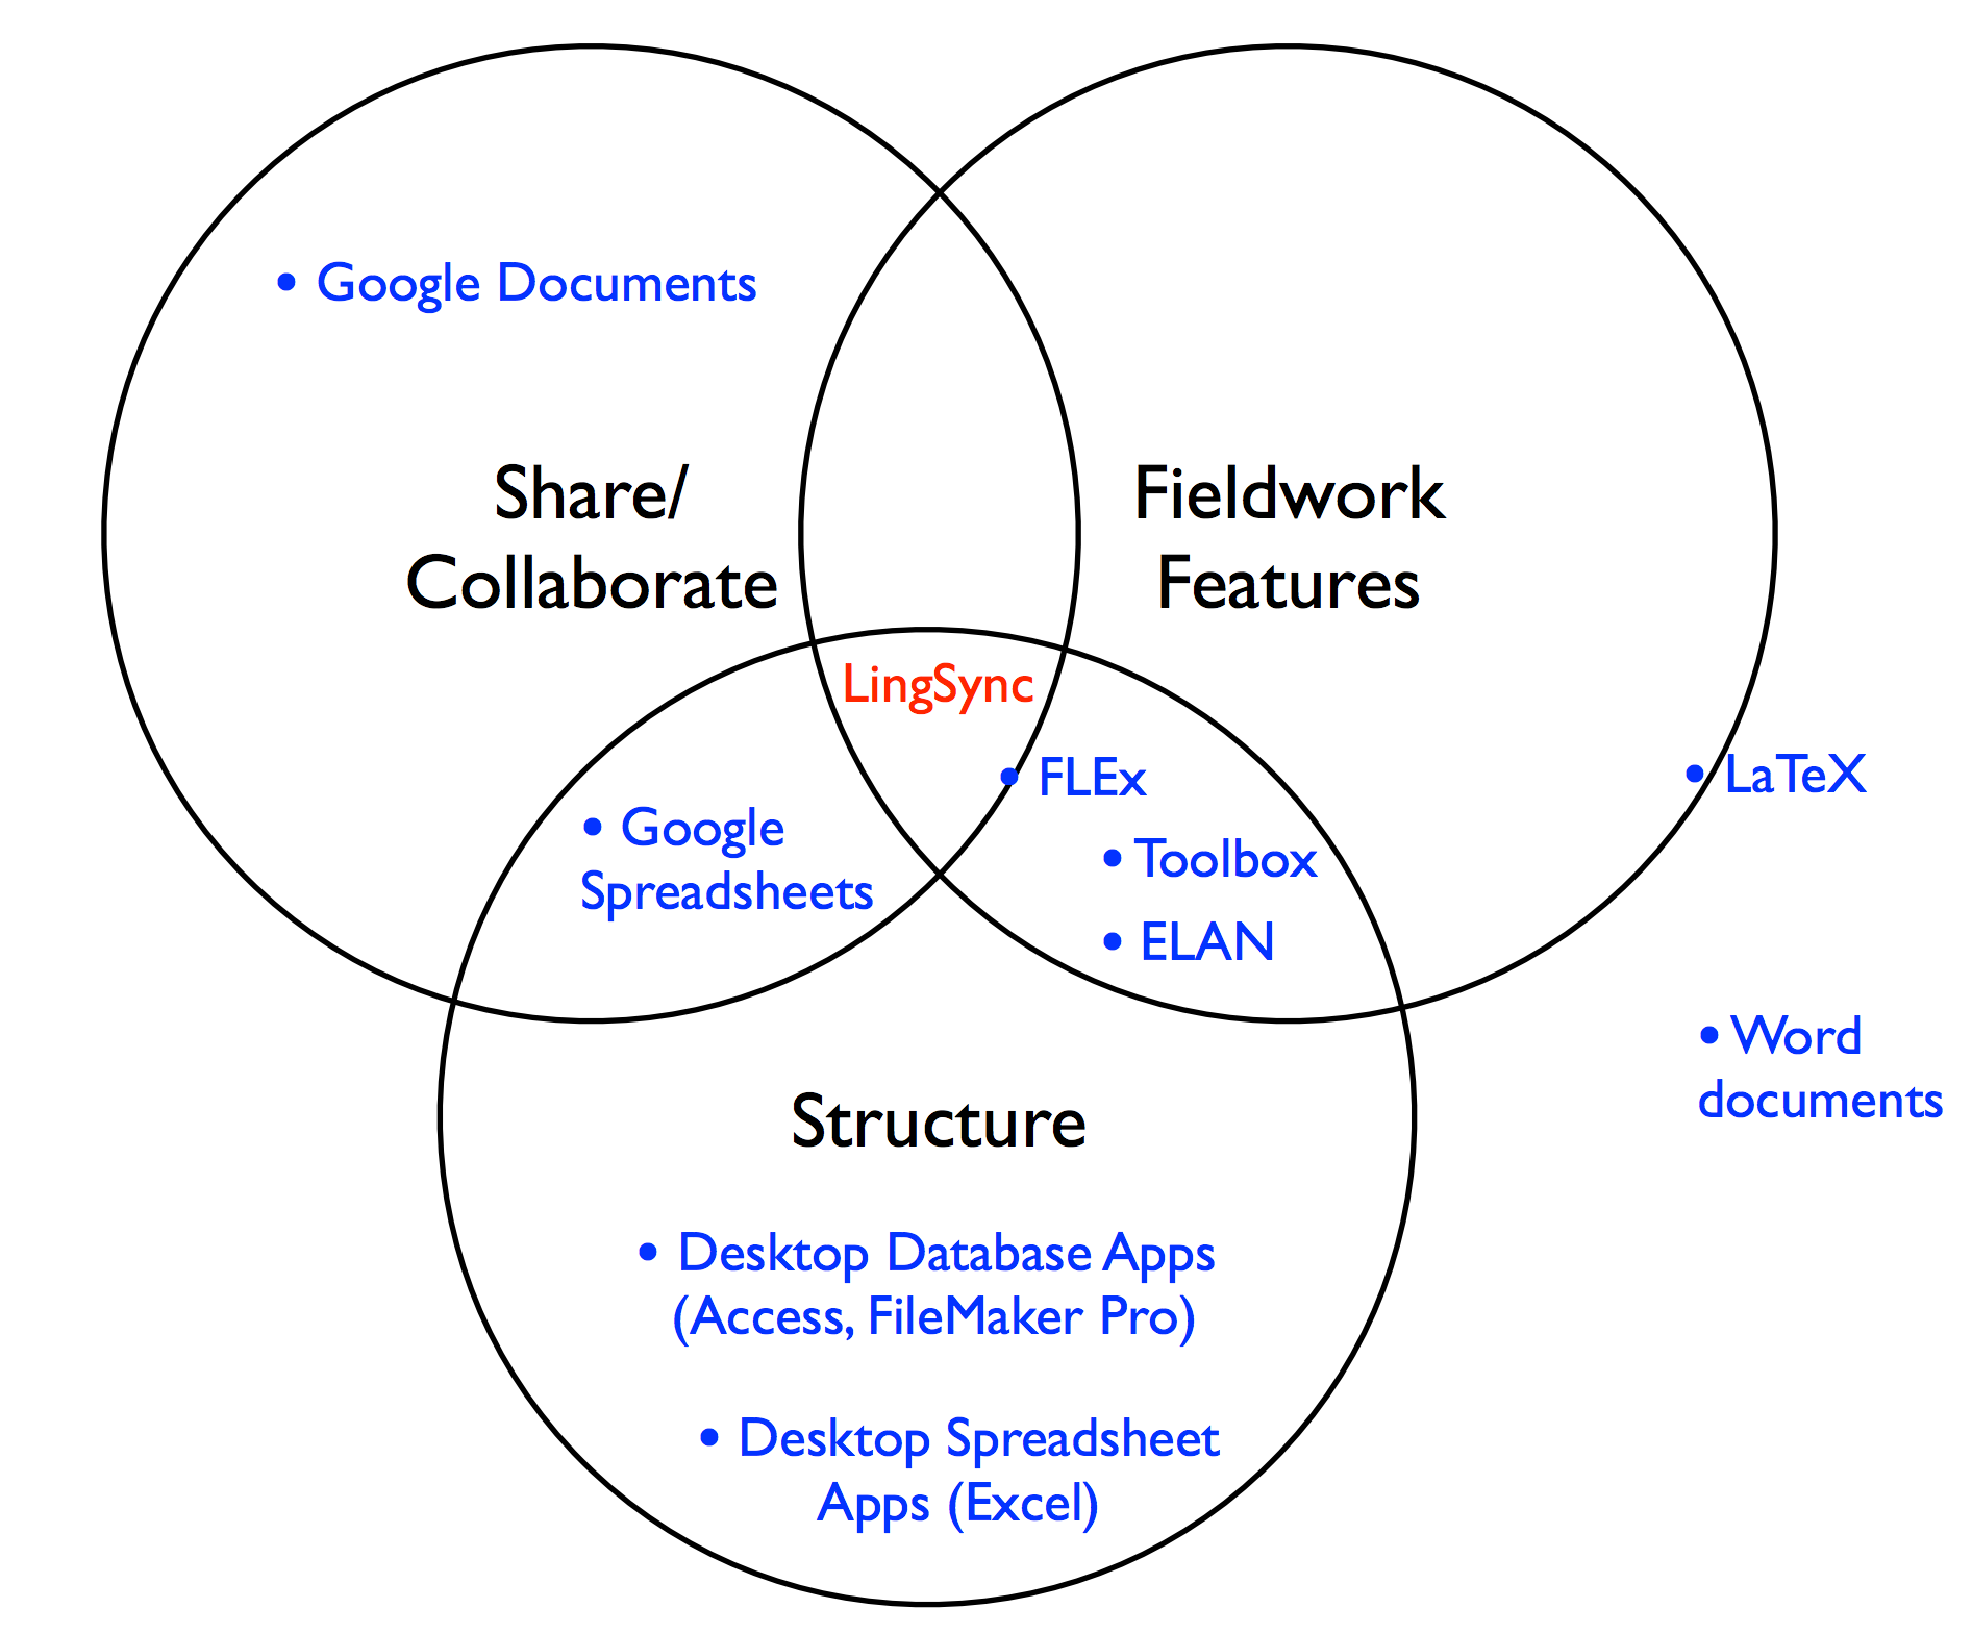
\includegraphics[width=3in]{../figures/other_software_sets}
\label{othersoftware}
\end{center}
\end{figure}

\end{frame}


\begin{frame}
%TODO will convert into latex diagrams once we are sure we want it.
\begin{figure}
\begin{center}
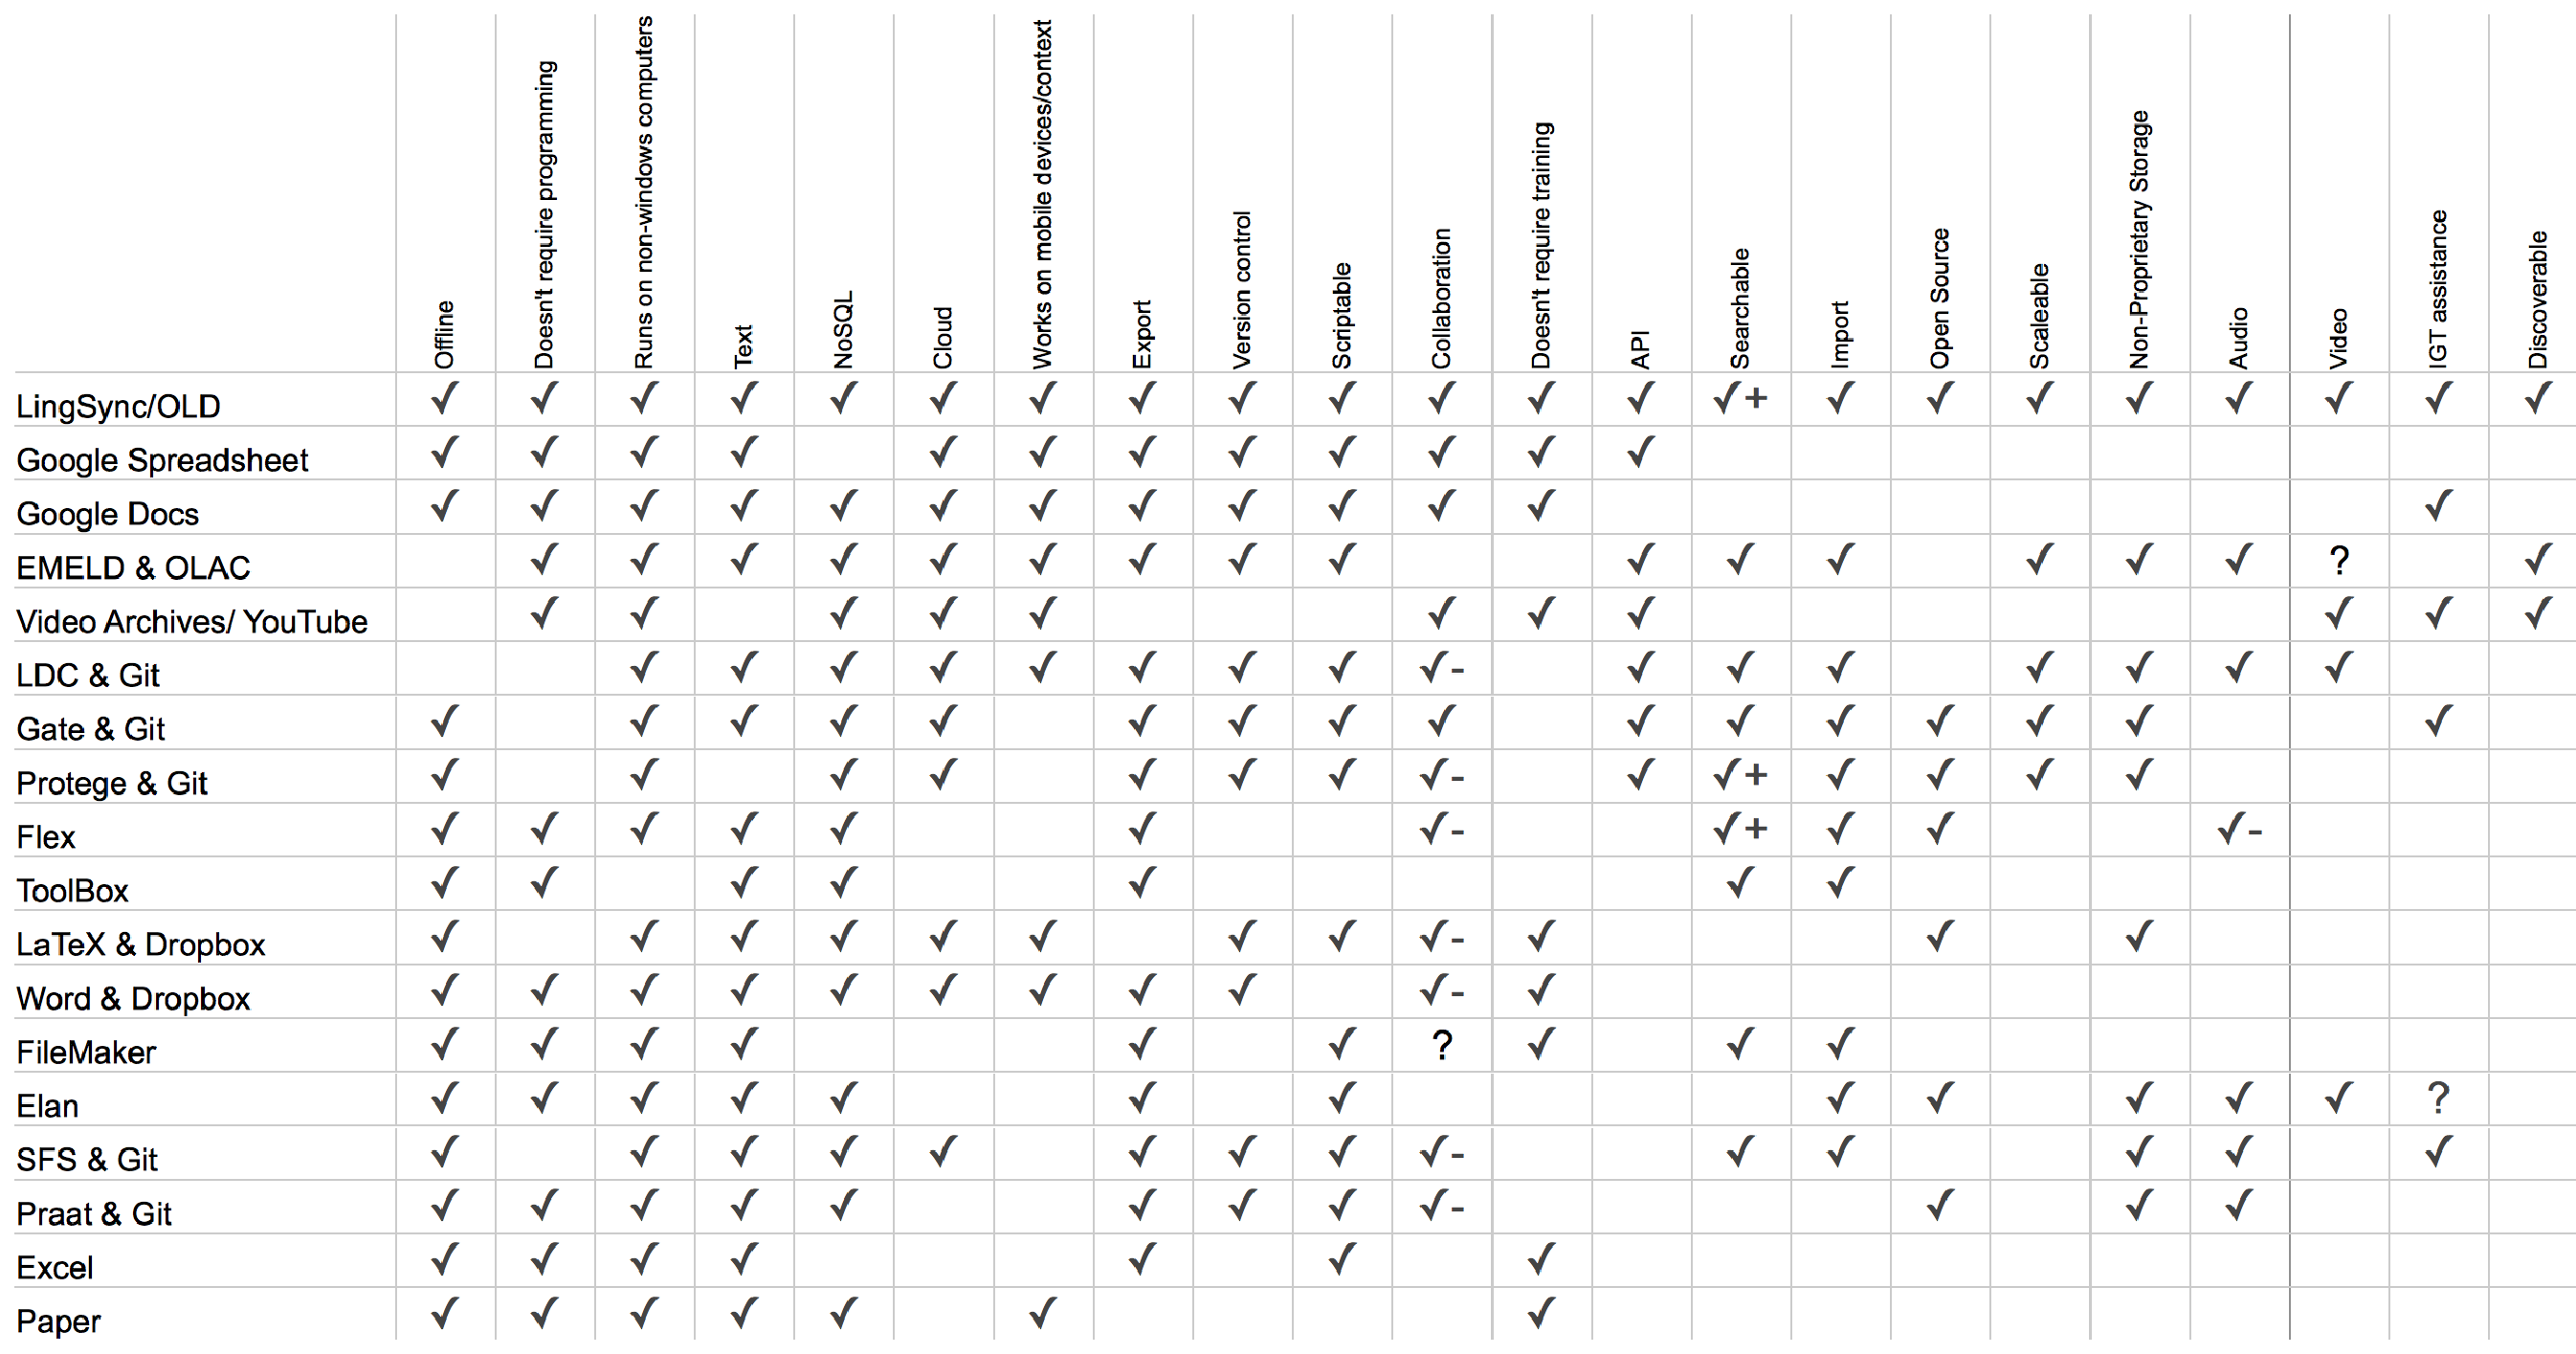
\includegraphics[width=3in]{../figures/other_software}
\caption{Many ad-hoc software combinations are used by teams.}
\label{allothersoftware}
\end{center}
\end{figure}
\end{frame}


\section[LingSync/OLD]{New models for data collection and management}
\subsection{LingSync}\label{sec:lingsync}


\begin{frame}
%TODO will convert into latex diagrams once we are sure we want it.
\begin{figure}
\begin{center}
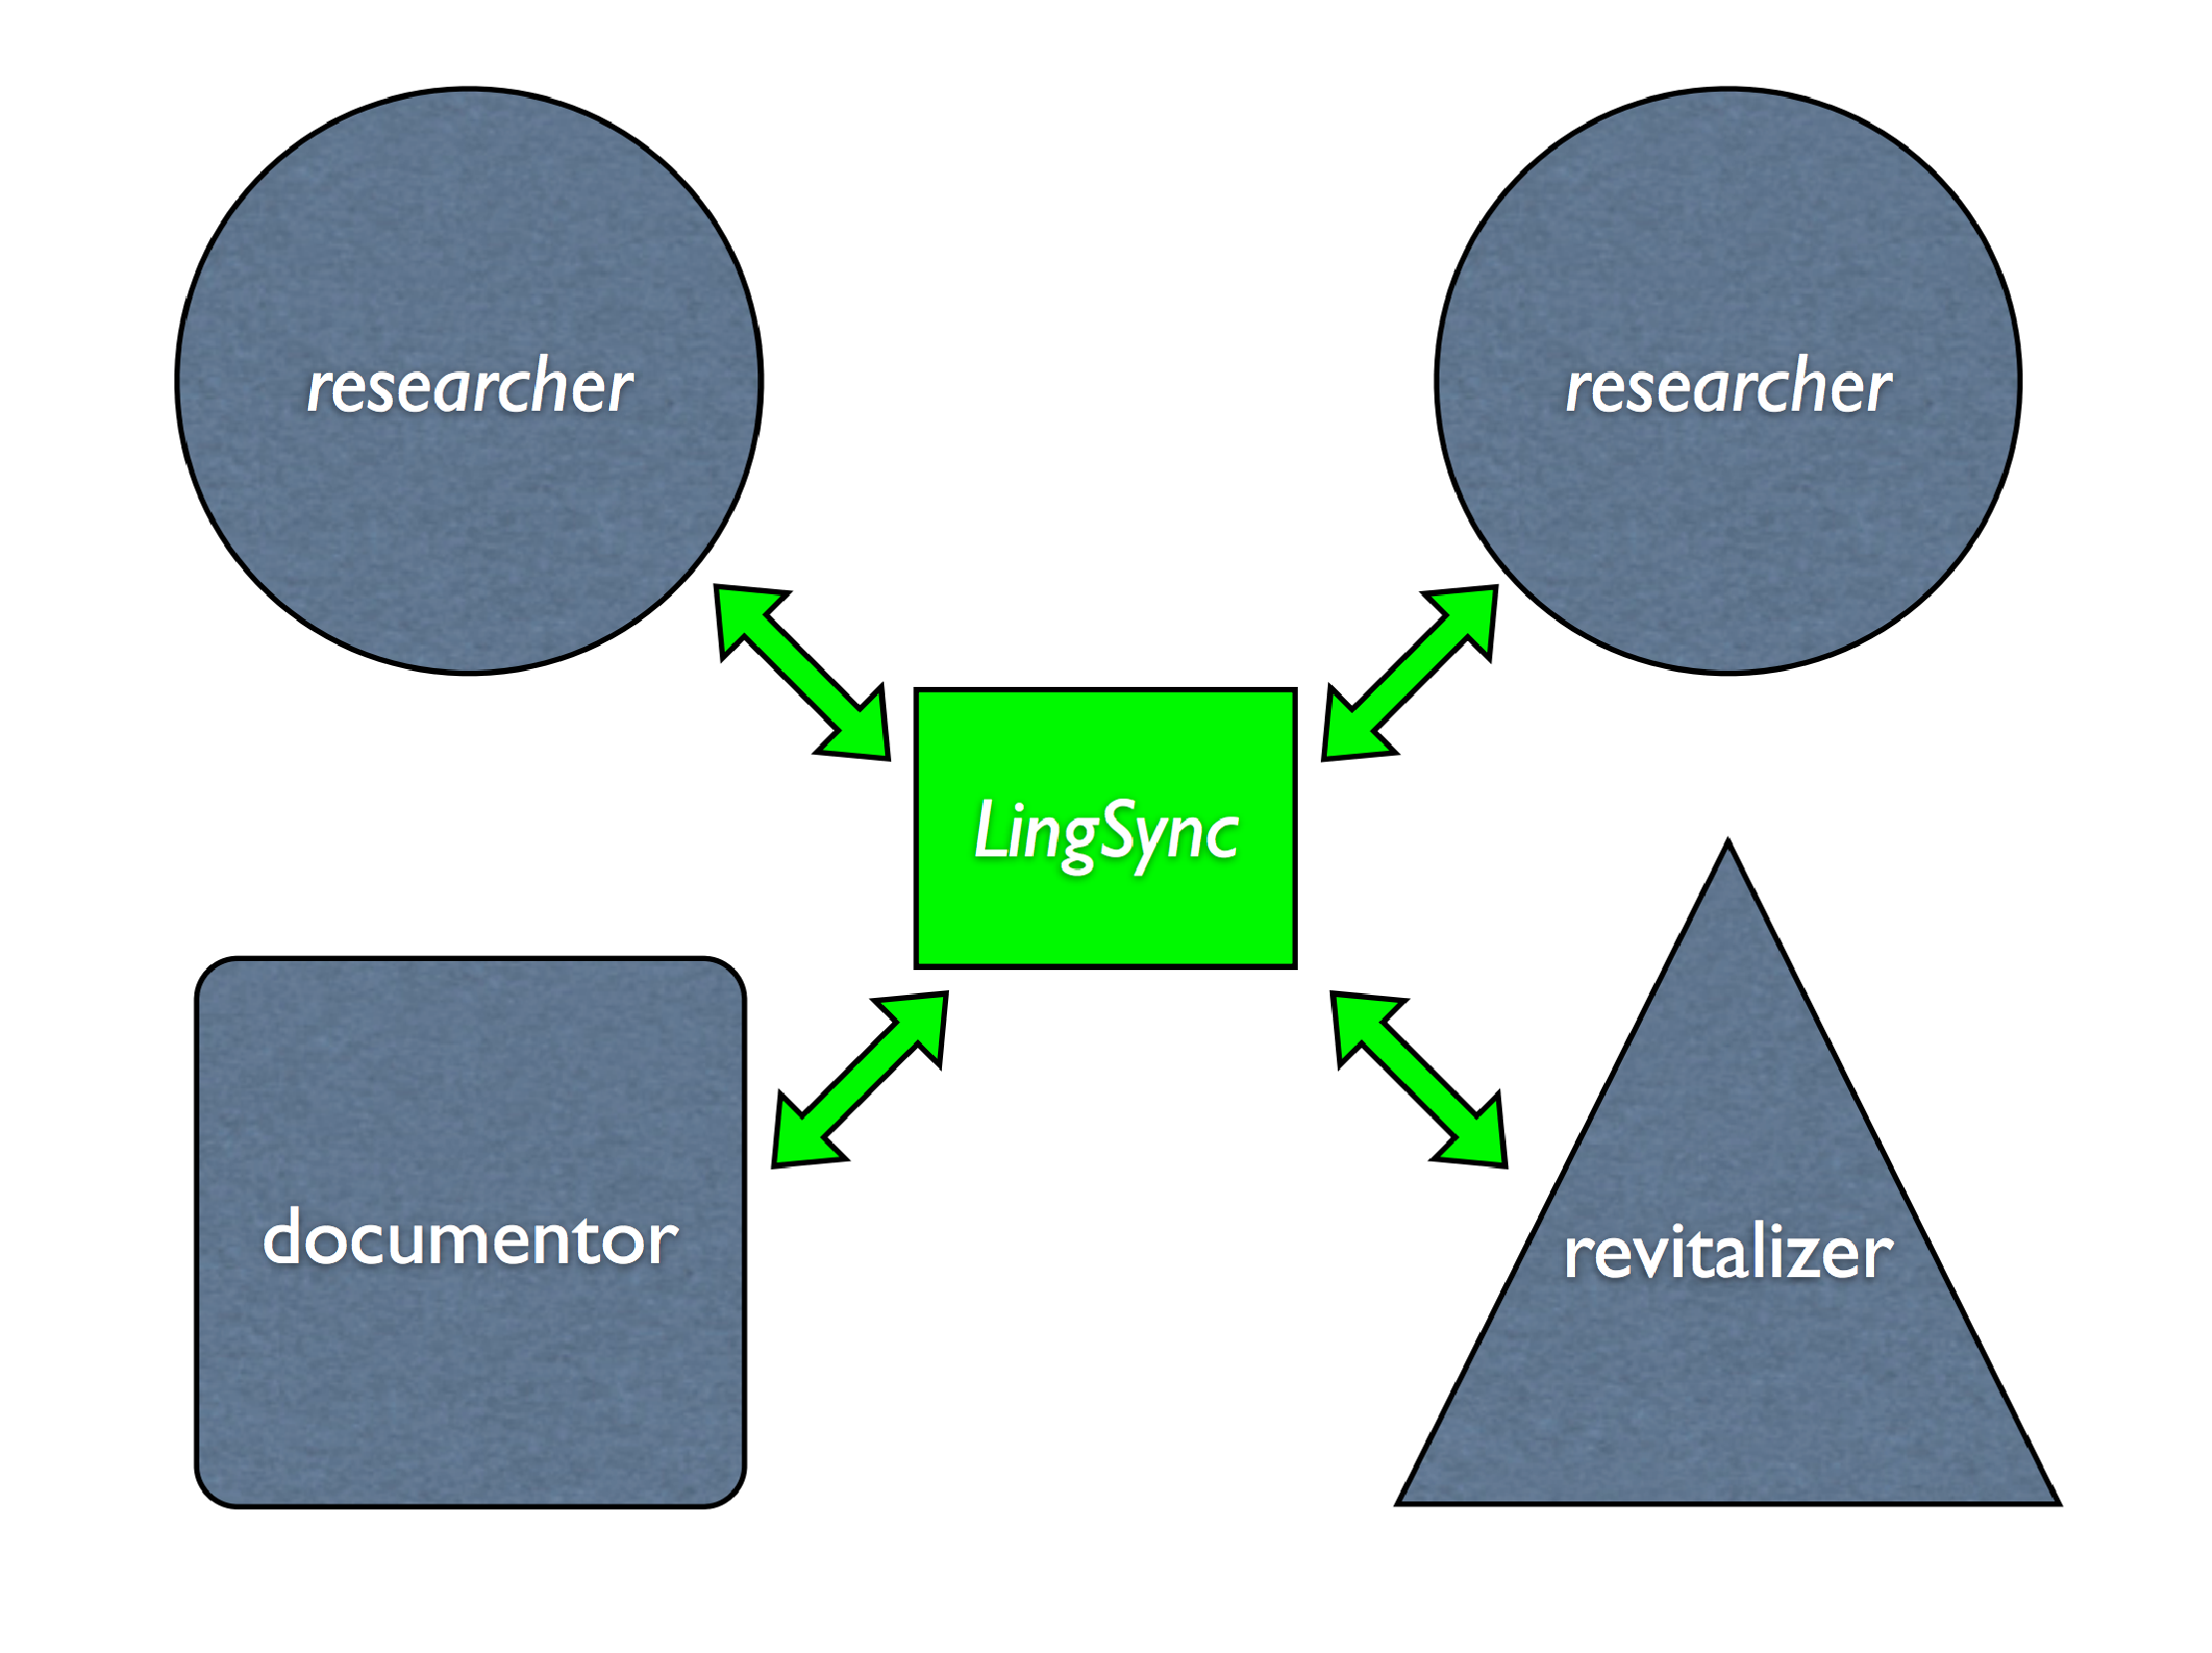
\includegraphics[width=3in]{../figures/bridge_stakeholders}
\label{lingsync:bridge}
\end{center}
\end{figure}
\end{frame}



\begin{frame}
%TODO will convert into latex diagrams once we are sure we want it.
\begin{figure}
\begin{center}
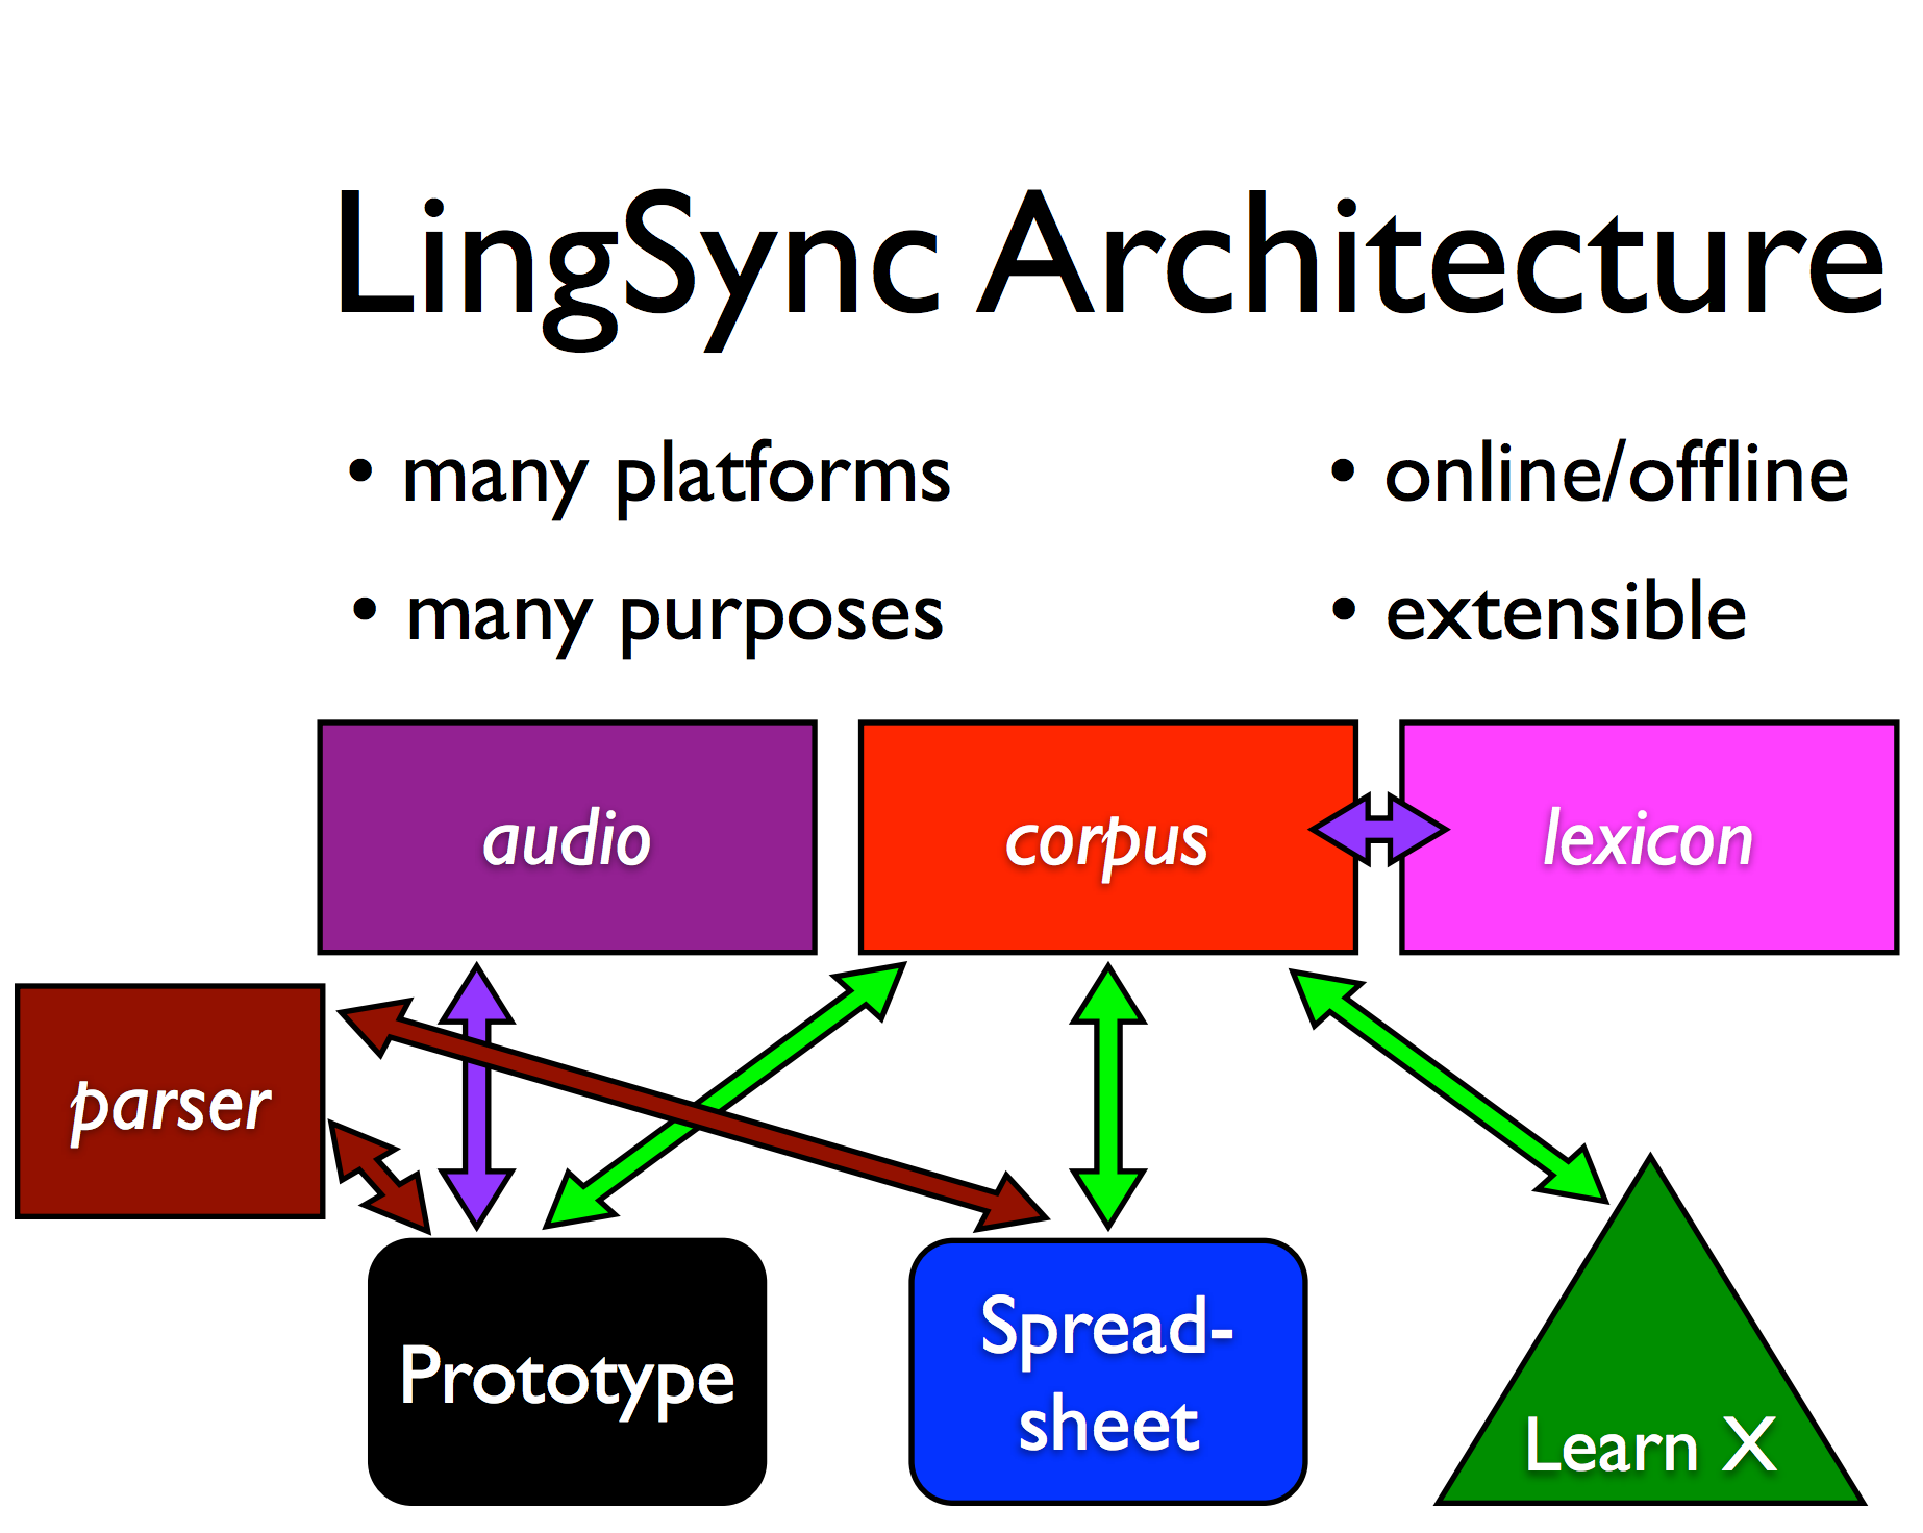
\includegraphics[width=3in]{../figures/architecture}
\label{lingsync:architecture}
\end{center}
\end{figure}
\end{frame}


\begin{frame}
%TODO will convert into latex diagrams once we are sure we want it.
\begin{figure}
\begin{center}
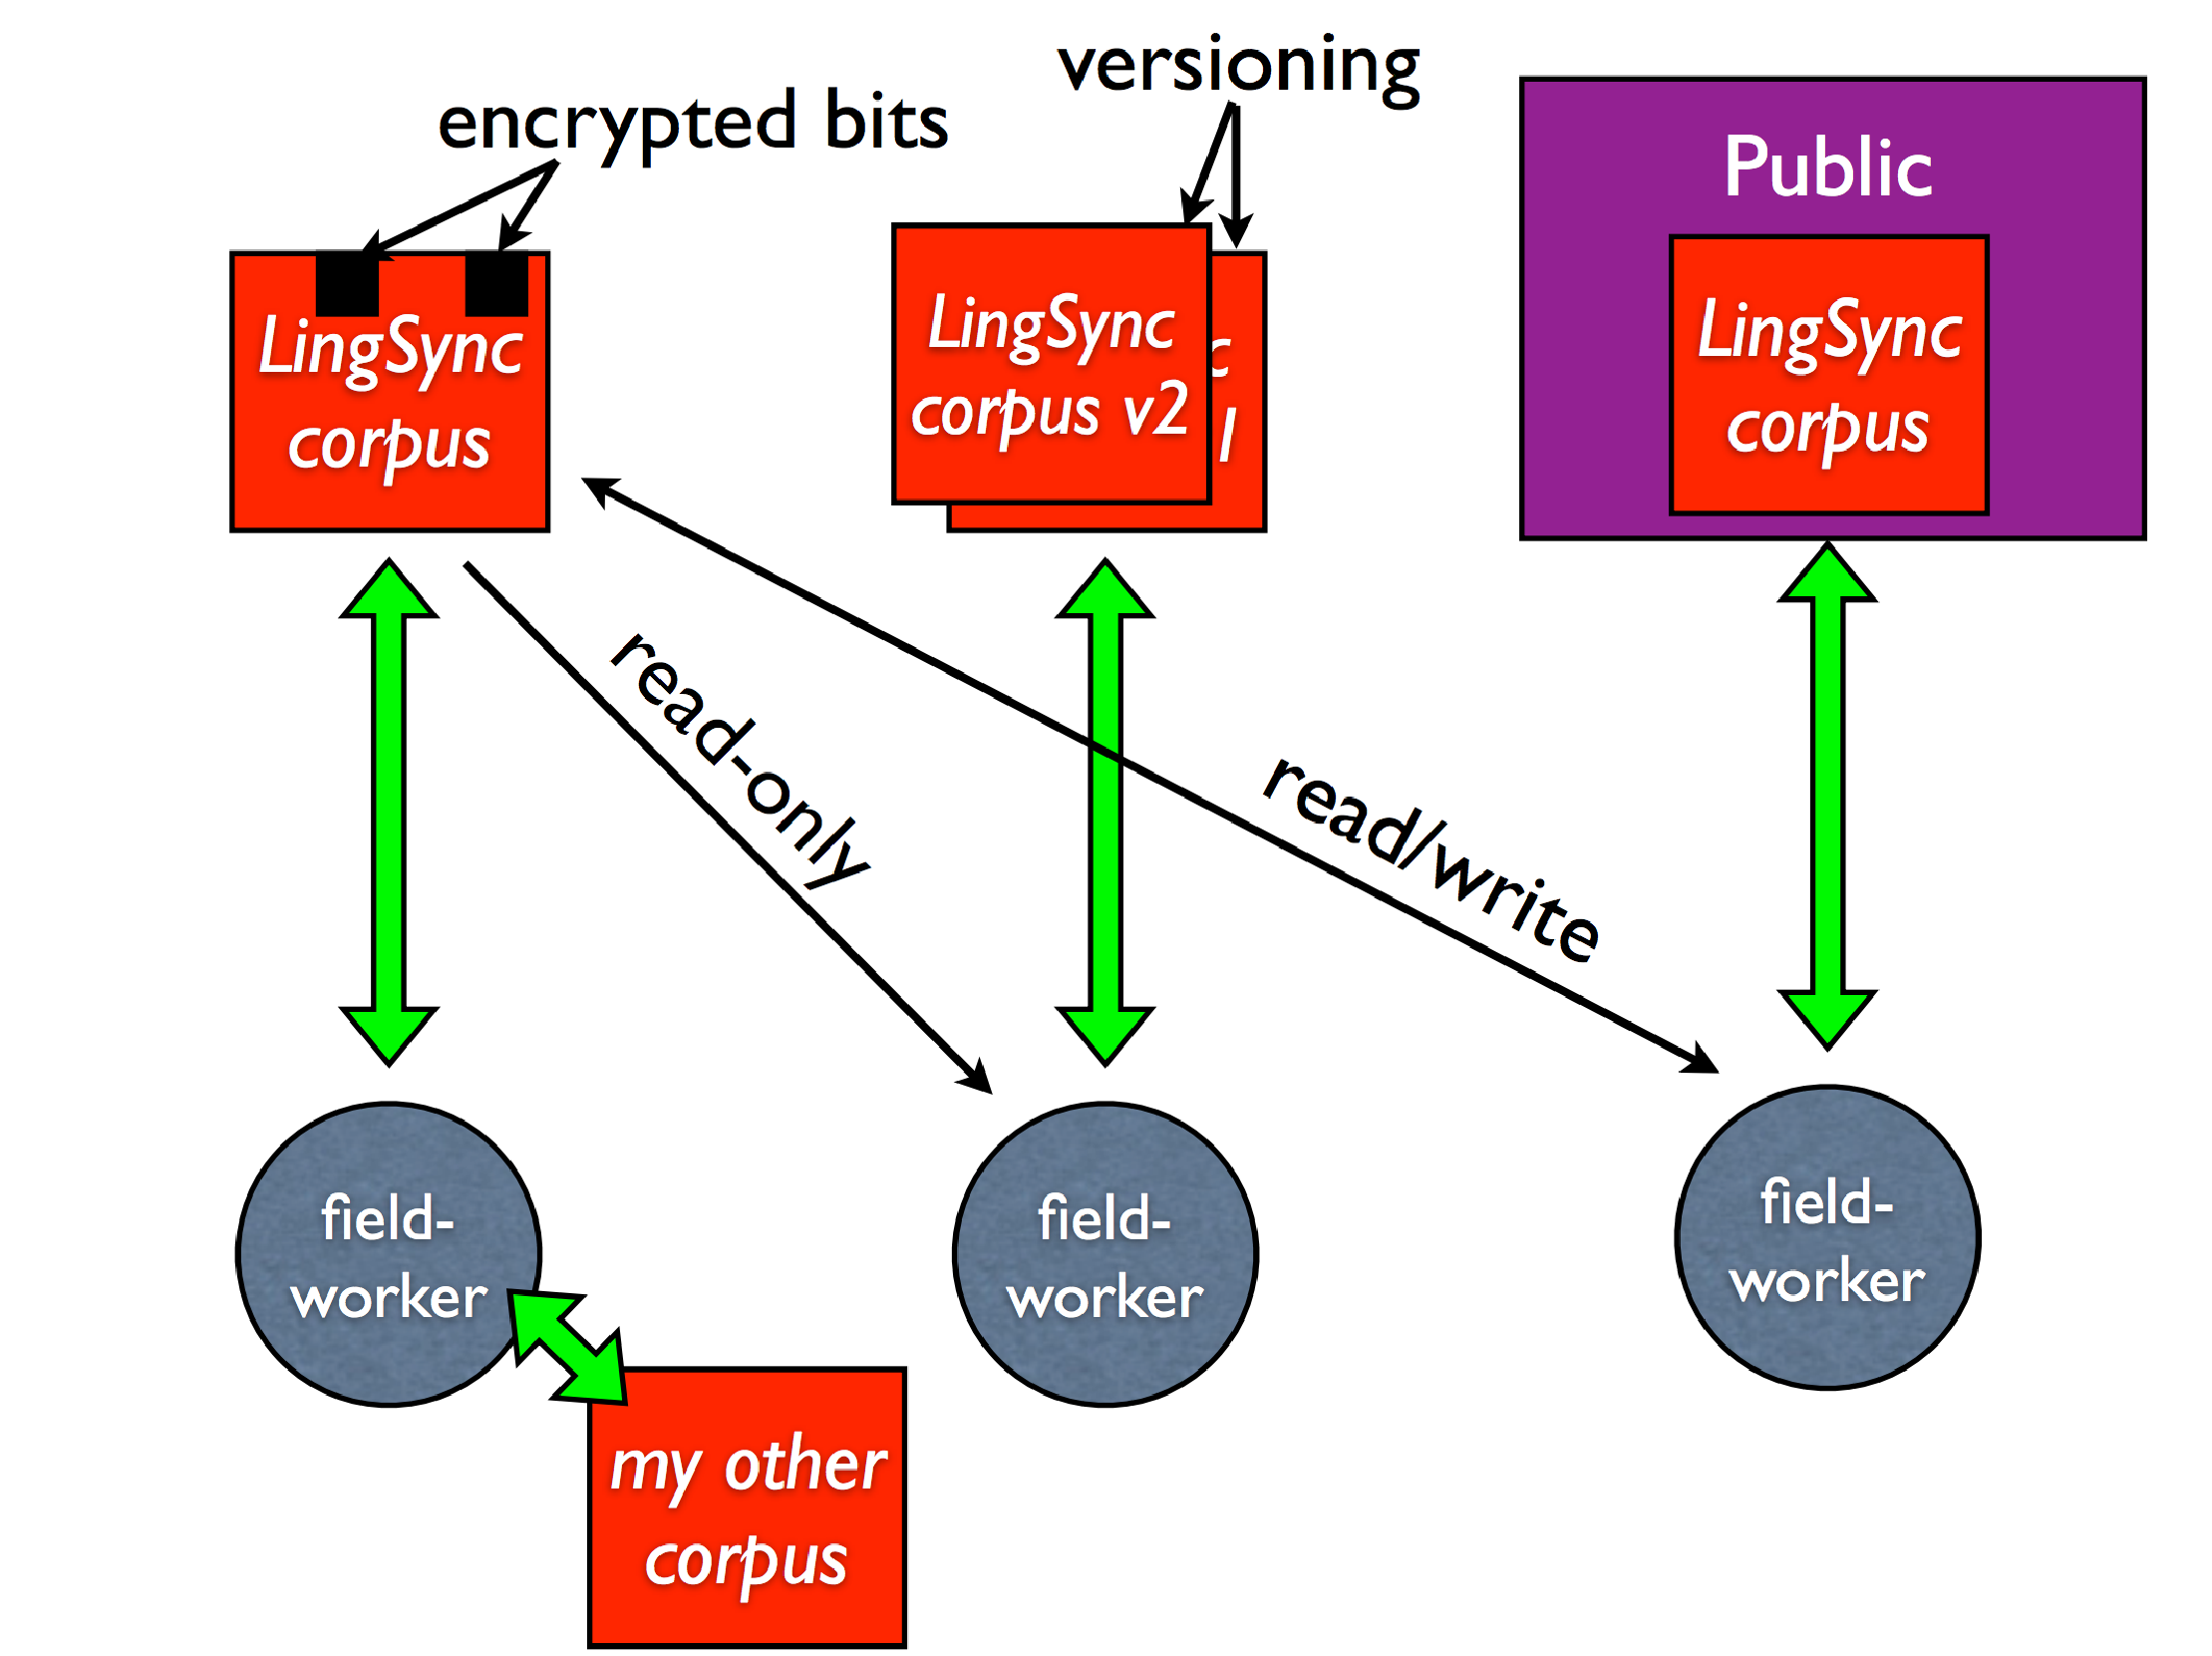
\includegraphics[width=3in]{../figures/corpora}
\label{lingsync:corpora}
\end{center}
\end{figure}
\end{frame}

\subsection{OLD}\label{sec:old}

\begin{frame}
OLD
\end{frame}

%\subsection{LingSync/OLD}

\subsection{User adoption}

\begin{frame}

\begin{table}[h]
\begin{center}
\scriptsize
\begin{tabular}{lrrrr}
      \toprule
                     ~ &  Active & Investigating & In-active & Total\\
      \midrule
      Public Corpora  &       2 &   1 &   2 & 5 \\ 
      Private Corpora &      15 &  37 & 321 & 373\\ 
      Users           &      38 &  43 & 220 & 301 \\
      Documents & 13,408 & 2,763 & 4,541 &23,487\\
      Disk Size & 1GB & .9GB & 5.3GB& 7.2GB\\
      
      \bottomrule

\end{tabular}
\caption{Data in LingSync corpora (Feb 14, 2014). Active corpora: $>$300
activities; Investigating corpora: 300-10 activities; Active users: $>$100
activities; Investigating users: 100-10 activities.}
\label{lingsync-data}
 \end{center}
 \normalsize
\end{table}

\end{frame}


\begin{frame}

\begin{table}[h]
 \begin{center}
     \scriptsize
\begin{tabular}{lrrrrr}

      \toprule
      language &                     \emph{forms}  & texts & audio & GB   & speakers \\
      \midrule
      Blackfoot (\textit{bla}) &     8,847  & 171   & 2,057 & 3.8  & 3,350    \\ % 11,075 4047074461 bytes
      Nata (\textit{ntk}) &          3,219  & 32    & 0     & 0    & 36,000   \\ % 3,251  0 bytes
      Gitksan (\textit{git}) &       2,174  & 6     & 36    & 3.5  & 930      \\ % 2,216  3787227136 bytes
      Okanagan (\textit{oka}) &      1,798  & 39    & 87    & 0.3  & 770      \\ % 1,924  349478912 bytes
      Tlingit (\textit{tli}) &       1,521  & 32    & 107   & 12   & 630      \\ % 1,660  12906459136 bytes
      Plains Cree (\textit{crk}) &   686    & 10    & 0     & 0    & 260      \\ % 696    0 bytes
      Ktunaxa (\textit{kut}) &       467    & 33    & 112   & 0.2  & 106      \\ % 612    176128000 bytes
      Coeur d'Alene (\textit{crd}) & 377    & 0     & 199   & 0.0  & 2        \\ % 576    28659712 bytes
      Kwak'wala (\textit{kwk}) &     98     & 1     & 1     & 0.0  & 585      \\ % 100    7450624 bytes
      TOTAL &                        19,187 & 324   & 2,599 & 19.8 &         \\ % 22,110 21302477981 bytes
      \bottomrule

\end{tabular}
\caption{Data in OLD applications (Feb 14, 2014)}
\label{old-data}
 \end{center}
 \normalsize
\end{table}


\end{frame}

%\section[Data]{Using LingSync/OLD}\label{open-data}
%
%\begin{frame}
%Using LingSync/OLD
%\end{frame}


\section[Plugins]{Plugins \& Reusing existing tools and libraries}

\subsection{Audio}
\subsubsection[Alignment]{Audio-transcription alignment}

\begin{frame}
Audio-transcription alignment
\end{frame}


\subsubsection[ASR]{Speech Recognition for Information Retrieval}

\begin{frame}
Speech Recognition for Legal Search in Kartuli
\end{frame}


\subsection{Morphology}



\subsubsection[Existing]{Existing morphological parsers}

\begin{frame}
Existing morphological parsers
\end{frame}




\subsubsection[Statistical]{Semi-supervised morphological parsers}

\begin{frame}
Semi-supervised morphological parsers
\end{frame}




\subsubsection[Novel]{Novel morphological parsers}

\begin{frame}
Novel morphological parsers
\end{frame}




\section{The Take-Home}

\begin{frame}
Take Home
\end{frame}

\section*{(Team)}

\begin{frame}
Acknowledgements
\end{frame}



\begin{frame}
References
\end{frame}


\end{document}
